\documentclass[11pt]{article}

\usepackage{amsmath}
\numberwithin{equation}{section}
\usepackage{amssymb}
\usepackage{amsthm}
\usepackage{blindtext}
\usepackage[parfill]{parskip}
\usepackage{graphicx}
\usepackage{textcomp}
\usepackage[utf8]{inputenc}
\usepackage{float}
\usepackage{diagbox}
\usepackage{tikz}
\usepackage{pgfgantt}
\usepackage{nicefrac}
\usepackage{caption}
\usepackage{setspace}
\usepackage{geometry}
\usepackage[toc,page]{appendix}
\usepackage{lipsum}
\usepackage[export]{adjustbox}
\usepackage[T1]{fontenc}
\usepackage{textcomp}
\usepackage{epsfig,graphics}
\usepackage{titlesec}

\newcommand{\projectTitle}{Matrix Solvers for Stochastic Galerkin Schemes}
\newcommand{\fullname}{Alexander Harvey}
\newcommand{\degreeTitle}{MSc Advanced Computer Science}
\newcommand{\session}{2017/18}

\newcommand{\frontcover}{
% The title page:
\begin{titlepage}
\newgeometry{left=25mm,right=25mm,top=45mm,bottom=0.1cm}

\begin{minipage}[t]{7cm}
\noindent\textbf{\Large{School of Computing}}\\
{\fontfamily{ptm}\selectfont 
\uppercase{faculty of engineering}
}
\end{minipage}
\hfill
\begin{minipage}[t]{7cm}
\vspace*{-25pt}
\includegraphics[scale=0.2,right]{logo_black.png}
\vspace*{-1pt}
\end{minipage}

\noindent\makebox[\linewidth]{\rule{\paperwidth}{0.4pt}}

\centering
\vspace*{37mm}
\textbf{\Large\projectTitle}\\
\vspace*{10mm}
\textbf{\large\fullname}\\
\vspace*{10mm}
\textbf{Submitted in accordance with the requirements for the degree of}\\
\textbf{\degreeTitle}\\
\vspace*{10mm}
\session\\
\restoregeometry
\end{titlepage}
}

\newcommand{\subsubsubsection}[1]{\paragraph{#1}\mbox{}\\}
\setcounter{secnumdepth}{4}
\setcounter{tocdepth}{4}

\onehalfspacing

\begin{document}

\frontcover

\newpage

\tableofcontents

\clearpage

\section{Introduction}
This project involves exploring methods for solving matrix equations that arise from partial differential equations (PDEs) and how a problem's structure can be exploited when dealing with equations in this form. This is not often the case when using conventional methods to solve PDEs, which usually involve stacking the unknowns of a problem into a single vector. The project then goes on to investigate how the methods explored can be applied to stochastic PDEs (PDEs with uncertain input). We begin by constructing the matrix form of Poission's equation.

\subsection{Possion Equation}
As an example, define spatial domain $\mathcal{D} = \{(x,y) : 0 \leq x \leq 1, \; 0 \leq y \leq 1 \}$ and let $u: \mathcal{D} \to \mathbb{R}$ be the solution of Poisson's equation:
	\begin{alignat}{1} 
	-u_{xx} - u_{yy} = {} & f \quad \text{ on } \mathcal{D} \nonumber \\
	u = {} & 0 \quad \text{ on } \partial \mathcal{D}
	\end{alignat}
as shown in Figure 1.

\begin{figure}[H]
\begin{tikzpicture}
\draw (0,0) rectangle (6,6);
\node at (3,3) {$-u_{xx}-u_{yy}=f$};
\node at (-0.25,3) {$0$};
\node at (6.25,3) {$0$};
\node at (3,-0.25) {$0$};
\node at (3,6.25) {$0$};

\node at (-0.25,-0.25) {$(0,0)$};
\node at (-0.25,6.25) {$(0,1)$};
\node at (6.25,-0.25) {$(1,0)$};
\node at (6.25,6.25) {$(1,1)$};

\draw[->] (7,0) -- (8,0);
\draw[->] (7,0) -- (7,1);
\node at (7.5,-0.25) {$x$};
\node at (6.75,0.5) {$y$};
\end{tikzpicture}
\centering
\caption{Domain for $-u_{xx}-u_{yy}=f$.}
\end{figure}

The domain of this PDE can be discretised into a mesh with uniform spacing $h$ using the centred finite difference approximations:
	\begin{equation} 
	u_{xx} \approx \frac{u_{i-1j} - 2u_{ij} + u_{i+1j}}{h^2}
	\end{equation}
	\begin{equation}
	u_{yy} \approx \frac{u_{ij-1} - 2u_{ij} + u_{ij+1}}{h^2}
	\end{equation}
where $u_{ij} = u(x_i, y_j)$. The mesh is shown in Figure 2.

\begin{figure}[H]
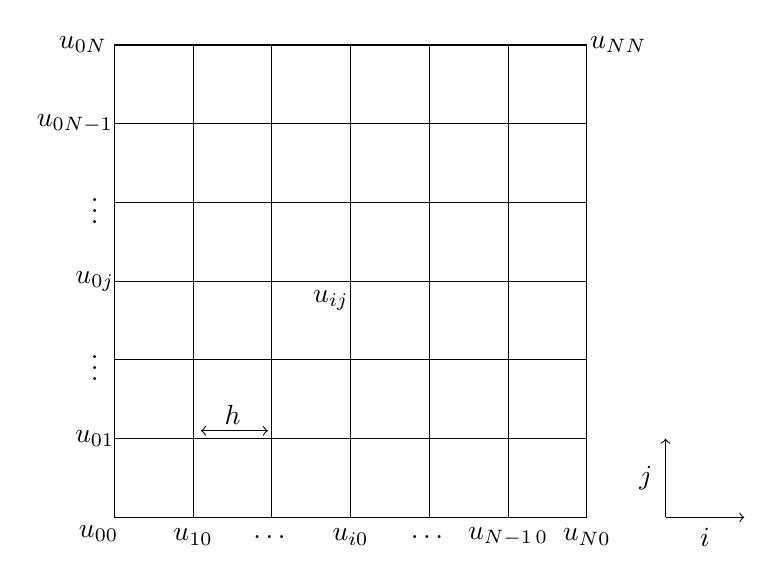
\begin{tikzpicture}
\draw (0,0) grid (6,6);
\node at (-0.2,-0.2) {$u_{00}$};
\node at (1,-0.25) {$u_{10}$};
\node at (2,-0.25) {$\dots$};
\node at (3,-0.25) {$u_{i0}$};
\node at (4,-0.25) {$\dots$};
\node at (5,-0.25) {$u_{N-1\,0}$};
\node at (6,-0.25) {$u_{N0}$};

\node at (-0.25,1) {$u_{01}$};
\node at (-0.25,2) {$\vdots$};
\node at (-0.25,3) {$u_{0j}$};
\node at (-0.25,4) {$\vdots$};
\node at (-0.5,5) {$u_{0N-1}$};
\node at (-0.4,6) {$u_{0N}$};

\node at (2.75,2.75) {$u_{ij}$};
\node at (6.4,6) {$u_{NN}$};

\draw[->] (7,0) -- (8,0);
\draw[->] (7,0) -- (7,1);
\node at (7.5,-0.25) {$i$};
\node at (6.75,0.5) {$j$};

\draw[<->] (1.1,1.1) -- (1.95,1.1);
\node at (1.5,1.3) {$h$};

\end{tikzpicture}
\centering
\caption{Discretised domain for $-u_{xx}-u_{yy}=f$.}
\end{figure}

The discretised form of this PDE can then be solved by computing the equation:
	\begin{equation}
	f_{ij} = -\frac{1}{h^2} \big( u_{i-1j} - 2u_{ij} + u_{i+1j} \big) - \frac{1}{h^2} \big( u_{ij-1} - 2u_{ij} + u_{ij+1} \big)
	\end{equation}
at each internal grid point, meaning the system has $n^2$ unknowns with $n=N-2$. The traditional approach to solving this discretised form would be to write (1.4) as:
	\begin{equation}
	f_{ij} = -\frac{1}{h^2} \big( u_{i-1j} + u_{ij-1} - 4u_{ij} + u_{i+1j} + u_{ij+1}  \big)
	\end{equation}
and then stack all unknowns $u_{ij}$ into a single vector $U$, resulting in the linear system $AU=F$. 

\subsection{Sylvester Equation}
A Sylvester equation is a matrix equation of the form $AX + XB = C$, where $A$ is a $n \times n$ matrix, $B$ is a $m \times m$ matrix, and $X$ and $C$ are $n \times m$ matrices. We can write (1.4) as a Sylvester equation in the form:
	\begin{equation}
	TU + UT = F
	\end{equation}
where $T$, $U$ and $F$ are of size $n \times n$.

Let $\text{tridiag}(j,i,k)$ be defined as a tridiagonal matrix with $i$ on the main diagonal and $j$ and $k$ on the left and right diagonals, respectively. Then for (1.6) we have $T=-\frac{1}{h^2} \, \text{tridiag}(1,-2,1)$ and $U_{ij} = u(x_i, y_j)$, where $(x_i, y_j)$ are interior grid nodes for $i,j=1,\dots,n$. The system has $n$ unknowns in each direction meaning there is a total of $n^2$ unknowns. The matrix equation is visualised below:
\begin{eqnarray}
\frac{-1}{h^2} 
\begin{pmatrix}
-2 & 1 & 0 & \dots & 0 & 0 \\
1 & -2 & 1 & \dots & 0 & 0 \\
0 & 1 & -2 & \dots & 0 & 0 \\
\vdots & \vdots & \vdots & \ddots & \vdots & \vdots \\
0 & 0 & 0 & \dots & -2 & 1 \\
0 & 0 & 0 & \dots & 1 & -2 \\
\end{pmatrix}
\begin{pmatrix}
u_{11} & u_{12} & \dots & u_{1j} & \dots & u_{1n} \\
u_{21} & u_{22} & \dots & u_{2j} & \dots & u_{2n} \\
\vdots & \vdots & \ddots & \vdots & \dots & \vdots \\
u_{i1} & u_{i2} & \dots & u_{ij} & \dots & u_{in} \\
\vdots & \vdots & \vdots & \vdots & \ddots & \vdots \\
u_{n1} & u_{n2} & \dots & u_{nj} & \dots & u_{nn}
\end{pmatrix} \nonumber \\ \nonumber
+
\begin{pmatrix}
u_{11} & u_{12} & \dots & u_{1j} & \dots & u_{1n} \\
u_{21} & u_{22} & \dots & u_{2j} & \dots & u_{2n} \\
\vdots & \vdots & \ddots & \vdots & \dots & \vdots \\
u_{i1} & u_{i2} & \dots & u_{ij} & \dots & u_{in} \\
\vdots & \vdots & \vdots & \vdots & \ddots & \vdots \\
u_{n1} & u_{n2} & \dots & u_{nj} & \dots & u_{nn}
\end{pmatrix}
\frac{-1}{h^2} 
\begin{pmatrix}
-2 & 1 & 0 & \dots & 0 & 0 \\
1 & -2 & 1 & \dots & 0 & 0 \\
0 & 1 & -2 & \dots & 0 & 0 \\
\vdots & \vdots & \vdots & \ddots & \vdots & \vdots \\
0 & 0 & 0 & \dots & -2 & 1 \\
0 & 0 & 0 & \dots & 1 & -2 \\
\end{pmatrix}
= F
\end{eqnarray}
A variety of methods can now be used to solve this equation. These methods will be explored in Section 3. 

\subsection{Organisation}
The organisation of this report is as follows. Section 2 sets out the objectives and planning of the project. Section 3 explores different methods for solving Sylvester equations. Section 4 explores ways of solving stochastic PDEs. Section 5 studies an application problem that combines the knowledge gained in the previous sections. Finally, Section 6 is an evaluation of the project's success.

\newpage

\section{Scope and Schedule}
\subsection{Aim}
The aim of this project is to first study, implement and compare a range of matrix equation solvers. Following this, a specific problem will be derived with the help of my supervisor so that these solvers may be used and compared for a suitable application.

\subsection{Objectives}
The objectives of this project are as follows:
\begin{itemize}
\item To carry out an extensive, in-depth literature review on methods (both direct and iterative) for solving matrix equations from a wide range of sources. To decide which of these methods are appropriate to implement and to gain a solid understanding of how they work. 
\item To use and expand upon my programming experience to implement the chosen methods for solving matrix equations to solve the specified problem. 
\item To evaluate the implementation by comparing and contrasting the methods implemented to try to decide which is the best method for solving the given problem.
\item To derive a suitable application equation so that the methods studied in this project can be applied to a specific problem. 
\item To clearly present the work carried out during the project by using and building upon my report writing skills.
\end{itemize}

\subsection{Deliverables}
The deliverables of this project include:
\begin{itemize}
\item The final report that will include the details of the matrix solvers that have been studied, how the solvers were implemented, an evaluation and comparison of the implemented solvers, an analysis of how these solvers were used to solve the chosen application problem, and finally an evaluation of the success of the project.  
\item Code that successfully implements the chosen matrix solvers so that they solve the given problem.
\end{itemize}

\subsection{Methodology}
The methodology of this project will first involve studying academic publishings to gain an understanding of various methods for solving matrix equations. Python will be used as the programming language of choice for the implementation because of my familiarity with it, the extensive amount of documentation available for it and the excellent libraries it has available (e.g. NumPy and SciPy). GitHub will be used for version control and the final report will be written using \LaTeX. 

\subsection{Tasks, Milestones and Timeline}
The steps of this project will be divided into iterations, with the problem in each iteration becoming successively more complex and difficult to solve. This is because understanding is a key part of this project, and so each iteration will build on the understanding of the last. Each iteration will consist of studying and applying matrix methods to the problem, implementing them in Python to solve the problem, evaluating the results and write up. Also rough deadlines will be given for when each iteration should be completed by, to ensure the project is on track at any given stage.

The iterations are as follows:
\begin{itemize}
\item Introductory problem: $-u_{xx} - u_{yy} = 2 \pi^2 \sin{(\pi x)} \sin{(\pi y)}$ - deadline June 1st
\item Problem introducing uncertainty: $-\varepsilon u_{xx} - \varepsilon u_{yy} = 2 \pi^2 \sin{(\pi x)} \sin{(\pi y)}$ - deadline June 22nd
\item A Poisson equation on a surface defined by a height map (not yet derived) - deadline July 13th
\item Application reaction-diffusion equation (not yet derived) - deadline August 3rd
\end{itemize}

If the project deadlines are met the remaining time will be dedicated to project evaluation, write up and any possible project extensions.

\newpage

\section{Matrix Solvers}
This section explores different methods for solving a particular matrix equation in Sylvester form. For spatial domain $\mathcal{D} = \{(x,y) : 0 \leq x \leq 1, \; 0 \leq y \leq 1 \}$ and $u: \mathcal{D} \rightarrow \mathbb{R}$, let $u(x,y) = \sin{(\pi x)} \sin{(\pi y)}$ be the exact solution of the equation:
\begin{alignat}{2}
-u_{xx} -u_{yy} = {} & f \quad & \text{ on } \mathcal{D} \nonumber \\
u = {} & 0 \quad & \text{ on } \partial \mathcal{D}
\end{alignat}
This gives:
\begin{equation}
\begin{split}
u_{xx} = u_{yy} = - \pi^2 \sin{(\pi x)} \sin{(\pi y)} \\
\implies f = 2 \pi^2 \sin{(\pi x)} \sin {(\pi y)}
\end{split}
\end{equation} 
The equation to be be solved is therefore:
\begin{alignat}{1}
-u_{xx} -u_{yy} = {} & 2 \pi^2 \sin{(\pi x)} \sin {(\pi y)} \quad \text{ on } \mathcal{D} \nonumber \\
u = {} & 0 \quad \text{ on } \partial \mathcal{D}
\end{alignat}
Using the centred finite difference approximations with uniform grid spacing $h$ to discretise the domain of this system, we have:
	\begin{equation}
	\begin{split}
	-\frac{1}{h^2} \big( u_{i-1j} - & 2u_{ij} + u_{i+1j} \big) - \frac{1}{h^2} \big( u_{ij-1} - 2u_{ij} + u_{ij+1} \big) 
	\\ & = 2\pi^2 \sin(\pi x_i) \sin(\pi y_j)
	\end{split}
	\end{equation}
to be solved at each grid point for $i, j = 1, \dots n$, where $n$ is the total number of unknowns in each direction. The matrix form of this equation is therefore:
\begin{equation}
	TU + UT = F
\end{equation}
where $T=-\frac{1}{h^2} \, \text{tridiag}(1,-2,1)$, $U_{ij} = u(x_i, y_j)$ and $F_{ij} = 2 \pi^2 \sin(\pi x_i) \sin(\pi y_j)$ are all matrices of size $n \times n$ and $(x_i, y_j)$ are interior grid nodes for $i,j=1,\dots,n$. This form allows us to explore different methods for solving this equation and compare them to the exact solution $u = \sin(\pi x) \sin(\pi y)$. A plot of the exact solution, with $n=1000$, is given in Figure 3. 
\begin{figure}[H]
\includegraphics[scale=.5]{img/solution2.png}
\centering
\caption{Plot of the solution with $n=1000$.}
\end{figure} 

Throughout the following section, each of the implemented methods will be given a maximum execution time of 6000 seconds to compute a solution. If a method does not compute a solution in this time for a certain problem size, then this will be specified in the results. If a method does not compute a solution because it needs more memory than is available, then this will also be specified. All tests in this section (and throughout the report) will be run on a DEC-10 computer with 32GB of RAM and 8 cores. 

The following measurements will be given to evaluate the performance of each of the methods implemented:
\begin{itemize}
\item $n$: The number of unknowns in each direction for the system - the total number of unknowns is $n^2$. The mesh size will be continually refined by a factor of $\frac{1}{2}$, meaning the total number of unknowns in each direction will be doubled at each level, until either the time limit is reached or too much memory is used. The starting value will be $n=125$, which will allow for a range of problem sizes to be tested without running more tests than necessary.
\item Time(s): The time taken in seconds for the method to compute the solution to the problem. As previously stated the maximum time allowed will be 6000 seconds.
\item $|| u - u_h ||_{L^\infty} $: An error measurement which measures the maximum difference between the actual solution and computed solution for each $u$. Defined as:
 \[ || u - u_h ||_{L^\infty} = \text{max}_{ij} | u(x_i, y_i) - u_{ij} | \]
\item $|| u - u_h ||_{L^2} $: An error measurement which measures the average difference between the actual solution and computed solution for all $u$, defined as:
\[ || u - u_h ||_{L^2} = \sqrt{h^2 \sum | u(x_i,y_j) - u_{ij} |^2} \]
\item Experimental order of convergence (eoc): Measures the rate of convergence of a method as the problem size is increased, which should approach 2 as the step size is increased. Defined as:
\[ \text{eoc}(i) = \frac{\log(\nicefrac{E_i}{E_{i-1}})}{\log(\nicefrac{h_i}{h_{i-1}})} \]
where $E_i$ is the error (chosen here as $|| u - u_h ||_{L^\infty}$) and $h_i$ is the mesh size at level $i$. 
\item Experimental order of growth (eog): Measures the order of growth of the execution time of an algorithm as the problem size is increased (that is, the approximate time complexity). Defined as:
\[ \text{eog}(i) = \frac{\log(\nicefrac{t_{i}}{t_{i-1}})}{\log(\nicefrac{n_{i}}{n_{i-1}})} \]
where $t_i$ is the total execution time and $n_i$ is the problem size at level $i$.
\item No. iters (iterative methods only): The number of iterations taken for the method to converge to the given convergence tolerance.
\end{itemize}
All non-integer measurements will be given to five significant figures. It is worth noting that as the total number of unknowns, and therefore the problem size, is $n^2$, the best time complexity that an optimal solver can achieve is $O(n^2)$, as it must compute a solution for each unknown. Also, as each of the methods is solving the same equation, the differences in error for each of the methods should be small.

\subsection{Direct Methods}

\subsubsection{Kronecker Product}
A naive approach to solving this equation is to use the Kronecker product to rewrite (3.5) as a standard vector linear system. The Sylvester equation $AX + XB = C$ can be written as the standard vector linear system:
\begin{equation}
\mathcal{A}x = c
\end{equation}
with $\mathcal{A} = I \otimes A + B^* \otimes I$, where $I$ is the identity matrix, $B^*$ denotes the conjugate transpose of $B$, $x = \text{vec}(X)$ and $c = \text{vec}(C)$.\footnote{The vec operator reshapes a matrix into a vector by stacking the columns one after another.}

The equivalent linear system for the matrix equation $TU + UT = F$ is:
\begin{equation}
\mathcal{T}u = \mathcal{F}
\end{equation}
where $\mathcal{F} = \text{vec}(F)$, $\mathcal{T} = I \otimes T + T \otimes I$ and $u = \text{vec}(U)$. 

This is the exact linear system that would be obtained from equation (1.5), that is, stacking all unknowns $u_{ij}$ into a single vector in the first place. Since the matrix $\mathcal{T}$ is sparse, this equation can be solved using a standard direct sparse solver. This approach provides a good base case for comparison. Results solving this linear system using the direct sparse solver \texttt{sparse.linalg.spsolve} from the SciPy library are shown in Table 1. As can be seen from the results, both errors decrease as the problem size $n$ is increased. The eoc is close to 2 for all $n$, demonstrating the convergence of the algorithm. As $n$ is increased the eog grows beyond $3$, which shows that this algorithm has worse than cubic time complexity for large $n$. For $n=4000$, this method results in a memory error. This is because \texttt{spsolve} tries to compute a (incomplete) LU decomposition of $\mathcal{T}$ which destroys the sparsity of the matrix and therefore requires much more memory to store it.

\begin{table}[H]
\centering
\begin{tabular}{|c|c|c|c|c|c|}
\hline
$n$ & Time(s) & $|| u - u_h ||_{L^{\infty}}$ &$|| u - u_h ||_{L^{2}}$ & eoc & eog \\
\hline
125 & 0.18141 & $5.1807 \times 10^{-5}$ & $2.5904 \times 10^{-5}$ & - & - \\
250 & 0.60371 & $1.3054 \times 10^{-5}$ & $6.5275 \times 10^{-6}$ & 2.0001 & 1.7346 \\
500 & 4.1663 & $3.2767 \times 10^{-6}$ & $1.6384 \times 10^{-6}$ & 1.9999 & 2.7868 \\
1000 & 36.113 & $8.2082 \times 10^{-7}$ & $4.1041 \times 10^{-7}$ & 2.0000 & 3.1157 \\
2000 & 404.48 & $2.0539 \times 10^{-7}$ & $1.0267 \times 10^{-7}$ & 2.0001 & 3.4855 \\
\cline{2-6}
4000 & \multicolumn{5}{c|}{Memory Error} \\
\hline
\end{tabular}
\captionsetup{justification=centering}
\caption{Results obtained from solving the linear system $\mathcal{A} x = c$ using the direct solver  \texttt{sparse.linalg.spsolve} from the SciPy library.}
\end{table}

\subsubsection{Bartels-Stewart Algorithm}
The Bartels-Stewart algorithm \cite{Bartels} can be used to solve the Sylvester equation $AX + XB = C$. 
This algorithm works by computing the Schur decompositions of the coefficient matrices $A$ and $B$, which are used to transform the equation into an equivalent form which has coefficient matrices which are upper and lower triangular, meaning it can be solved one element at a time. The solution of this triangular system is then used to obtain the solution to the original equation.

In the general case the algorithm is as follows:
\begin{enumerate}
\item Compute the Schur forms $A^* = PRP^*$ and $B=QSQ^*$.
\item Solve $R^*Y + YS = \hat{C}$ for $Y$, where $\hat{C} = P^*CQ$.
\item Compute $X=PYQ^*$.
\end{enumerate}
Here the matrices $R$ and $S$ are upper/lower triangular matrices with the eigenvalues of $A$ and $B$ on the diagonal, respectively. The matrices $P$ and $Q$ unitary matrices whose columns are orthonormal sets of eigenvectors obtained from the eigenvectors of $A$ and $B$, respectively.

By breaking this algorithm down into its component parts, we can examine each part to see which is the most costly. The first step of the algorithm can be computed using \texttt{linalg.schur} from the SciPy library, which uses the QR algorithm and has time complexity $O(n^3)$. For the second step, each entry of $Y$ can be computed as:
\begin{equation}
Y_{ij} = \hat{C}_{ij} - \sum_{p=1}^{i-1} R_{ip}Y_{pj} - \sum_{q=1}^{j-1} Y_{iq}S_{qj}
\end{equation}
for $i,j=1, \dots, n$. This also has time complexity $O(n^3)$, as it will have a \texttt{for} loop running from $i=1$ to $n$, a nested \texttt{for} loop running from $j=1$ to $n$ and then two nested \texttt{for} loops which run from $p=1$ and $q=1$ to $i-1$ and $j-1$, respectively. The last step of the algorithm is a simple matrix multiplication, which has time complexity of at most $O(n^3)$. Therefore we can expect this algorithm to run in roughly $O(n^3)$. 

The algorithm simplifies for $TU+UT=F$. In this case the algorithm is as follows:
\begin{enumerate}
\item Compute the Schur form $T=PRP^*$.
\item Solve $R^*V + VR = \hat{F}$ for $V$, where $\hat{F} =  P^*FP$.
\item Compute $U=PVP^*$.
\end{enumerate}
The first step now only requires a Schur decomposition of one matrix to be computed. The matrix $T$ is symmetric which means that its eigenvectors are orthogonal, which implies that $R$ is now a diagonal matrix which has the eigenvalues of $T$ on the diagonal. We can see this is true by examining the steps of the Schur decomposition. For a general matrix $A$, a Schur decomposition $A=PRP^*$ has 4 steps:
\begin{enumerate}
\item Find the eigenvalues of $A$.
\item Find the corresponding eigenvectors of $A$.
\item Compute an orthonormal set of eigenvectors using the eigenvectors of $A$, for example by using Gram-Schmidt orthogonalisation.
\item The eigenvectors found in Step 3 make up the columns of $P$. $R$ can now be found as $R=P^*AP$. 
\end{enumerate}
As the eigenvectors of $T$ are already orthogonal, they only need to be normalised in the 3rd step of the decomposition. This means that $R$ will be a diagonal matrix with the eigenvalues of $T$ on the diagonal.

This property reduces the complexity of the second step to $O(n^2)$, as only the diagonal elements need to be calculated and so the two summations are not necessary. We can therefore expect the algorithm to run faster than in the general case and to be dominated by the first step. We should therefore expect this algorithm to have, in the worst case, time complexity $O(n^3)$.

\subsubsection*{SciPy Solver}
The SciPy library has a built in solver for solving Sylvester equations, \texttt{linalg.solve \_sylvester}, which uses the Bartels-Stewart algorithm. We can use this to test the general algorithm. Results using this solver are given in Table 2. We can see from these results that the errors for this method are almost exactly the same as the errors in Table 1. Also this method is much faster and is able to solve a much larger problem size than using the Kronecker product. The eoc is close enough to 2 for all values of $n$ to conclude that this algorithm converges. The eog seems to change depending on the problem size, however for large $n$ has close to cubic time complexity. Although it is difficult to analyse the steps of this solver directly, \texttt{solve\_sylvester} makes use of LAPACK, an optimised software library for solving linear algebra problems, to compute the Schur decomposition in the first step. LAPACK uses a couple of different methods for computing the eigenpairs of symmetric tridiagonal matrices [\textbf{add reference}] and so it is likely that the method changes depending on the problem size, which causes the changes in the eog.

\begin{table}[H]
\centering
\begin{tabular}{|c|c|c|c|c|c|}
\hline
$n$ & Time(s) & $|| u - u_h ||_{L^{\infty}}$ &$|| u - u_h ||_{L^{2}}$ & eoc & eog \\
\hline
125 & 0.059959 & $5.1807 \times 10^{-5}$ & $2.5904 \times 10^{-5}$ & - & - \\
250 & 0.11421 & $1.3054 \times 10^{-5}$ & $6.5275 \times 10^{-6}$ & 2.0001 & 0.92964 \\
500 & 1.9383 & $3.2767 \times 10^{-6}$ & $1.6384 \times 10^{-6}$ & 1.9999 & 4.0850  \\
1000 & 4.0920 & $8.2084 \times 10^{-7}$ & $4.1042 \times 10^{-7}$ & 2.0000 & 1.0780 \\
2000 & 32.029 & $2.0503 \times 10^{-7}$ & $1.0259 \times 10^{-7}$ & 2.0027 & 2.9685  \\
4000 & 279.95 & $4.9949 \times 10^{-8}$ & $2.4876 \times 10^{-8}$ & 2.0377 & 3.1277  \\
8000 & 2812.2 & $8.6380 \times 10^{-9}$ & $4.1216 \times 10^{-9}$ & 2.5321 & 3.3285 \\
\cline{2-6}
16000 & \multicolumn{5}{c|}{Time Limit Reached} \\
\hline
\end{tabular}
\caption{Results using SciPy's \texttt{linalg.solve\_sylvester}.}
\end{table}

\subsubsection*{Simplified Implementation}

Results using the simplified version of this algorithm are shown in Table 3. These results demonstrate that this simplified implementation is much faster than the SciPy solver. The eoc demonstrates that this algorithm converges well up until $n=4000$, but after this point stops converging and when $n=16000$ the error becomes bigger than when $n=8000$. This is because \texttt{linalg.Schur} is used to compute the Schur decomposition in the first step, which uses the QR algorithm to approximate the eigenpairs of $T$ (as there is no general formula for calculating the eigenpairs of an arbitrary matrix). This approximation becomes less accurate as $n$ increases and for large $n$ has a significant impact on the solution. The eog here demonstrates that this algorithm has better than cubic time complexity.
\begin{table}[H]
\centering
\begin{tabular}{|c|c|c|c|c|c|}
\hline
$n$ & Time(s) & $|| u - u_h ||_{L^{\infty}}$ &$|| u - u_h ||_{L^{2}}$ & eoc & eog \\
\hline
125 & 0.036654 & $5.1807 \times 10^{-5}$ & $2.5904 \times 10^{-5}$ & - & - \\
250 & 0.084191 & $1.3054 \times 10^{-5}$ & $6.5275 \times 10^{-6}$ & 2.0001 & 1.1997 \\
500 & 0.35179 & $3.2766 \times 10^{-6}$ & $1.6383 \times 10^{-6}$ & 2.0000 & 2.0630 \\
1000 & 1.2846 & $8.2081 \times 10^{-7}$ & $4.1041 \times 10^{-7}$ & 2.0000 & 1.8685 \\
2000 & 7.3734 & $2.0531 \times 10^{-7}$ & $1.0265 \times 10^{-7}$ & 2.0007 & 2.5210 \\
4000 & 40.664 & $4.8578 \times 10^{-8}$ & $2.4421 \times 10^{-8}$ & 2.0802 & 2.4634 \\
8000 & 291.47 & $1.5975 \times 10^{-8}$ & $7.9337 \times 10^{-9}$ & 1.6048 & 2.8415 \\
16000 & 1797.2 & $1.6116 \times 10^{-7}$ & $9.0649 \times 10^{-8}$ & -3.3352 & 2.6243 \\
\cline{2-6}
32000 & \multicolumn{5}{c|}{Memory Error} \\
\hline
\end{tabular}
\caption{Results using the simplified Bartels-Stewart algorithm.}
\end{table}

Timing results of each step of the algorithm are given in Table 4, where the headings of the table correspond to each step of the algorithm. These results show that this algorithm is largely dominated by computing the Schur decompositions in the first step, as expected.

\begin{table}[H]
\centering
\begin{tabular}{|c|c|c|c|c|c|}
\hline
$n$ & 1 & 2 & 3 & Total & eog \\
\hline
125 & 0.023111 & 0.013408 & 0.00013494 & 0.036654 & - \\
250 & 0.035753 & 0.047841 & 0.00059700 & 0.084191 & 1.1997 \\
500 & 0.15627 & 0.19206 & 0.0034585 & 0.35179 & 2.0630 \\ 
1000 & 0.49460 & 0.76522 & 0.024728 & 1.2846 & 1.8685 \\
2000 & 3.1751 & 4.0314 & 0.16686 & 7.3734 & 2.5210 \\
4000 & 25.373 & 14.011 & 1.2787 & 40.664 & 2.4634 \\
8000 & 218.92 & 61.979 & 10.566 & 291.47 & 2.8415 \\
16000 & 1433.7 & 277.08 & 86.375 & 1797.2 & 2.6243 \\
\hline
\end{tabular}
\caption{Timings for each step using the simplified Bartels-Stewart algorithm.}
\end{table}

\subsubsection{Similarity Transformation}
A similarity transformation \cite{Simoncini} can be used to solve the Sylvester equation $AX + XB = C$. Assuming that the coefficient matrices $A$ and $B$ can be diagonalised, this method uses an eigendecomposition to reform the equation so that the solution can be easily obtained. The method is as follows:
\begin{enumerate}
\item Compute the eigendecompositions $P^{-1}AP = \text{diag}(\lambda_1, \dots, \lambda_n)$ and $Q^{-1}BQ = \text{diag}(\mu_1, \dots, \mu_m)$:
	\begin{enumerate}
	\item Compute the eigenpairs of $A$ and $B$
	\item Compute the inverses of $P$ and $Q$
	\end{enumerate}
\item Compute the solution $X = P \widetilde{X} Q^{-1}$, where $\widetilde{X}_{ij} = \frac{\widetilde{C}_{ij}}{\lambda_i + \mu_j}$ and $\widetilde{C} = P^{-1}CQ$.
\end{enumerate}
Here $\lambda_1, \dots, \lambda_n$ are the eigenvalues of $A$, $\mu_1, \dots, \mu_m$ are the eigenvalues of $B$ and the columns of $P$ and $Q$ are the eigenvectors of $A$ and $B$, respectively. We can analyse the steps of this algorithm as done previously to obtain the time complexity. Step 1a consists of computing the eigenpairs of $A$ and $B$, which in general is $O(n^3)$. Step 1b computes the inverse of $P$ and $Q$ which is greater than $O(n^2)$. The last step involves matrix multiplication which is at most $O(n^3)$. Therefore we can expect this algorithm in the general case to have, in the worst case, complexity $O(n^3)$, with the steps 1a and 2 dominating. 

For $TU+UT=F$ this method also simplifies. The steps are: 
\begin{enumerate}
\item Compute the eigendecomposition $P^{-1}TP = \text{diag}(\lambda_1, \dots, \lambda_n)$
	\begin{enumerate}
	\item Compute the eigenpairs of $T$
	\item Compute the inverse of $P$
	\end{enumerate}
\item Compute the solution $U = P \widetilde{U} P^{-1}$, where $\widetilde{U}_{ij} = \frac{\widetilde{F}_{ij}}{\lambda_i + \lambda_j}$ and $\widetilde{F}=P^{-1}FP$
\end{enumerate}
As before $\lambda_1, \dots, \lambda_n$ are the eigenvalues of $T$ and the columns of $P$ are the eigenvectors of $T$. The complexity of the first step can be drastically reduced. Here only one eigendecomposition needs to be performed. As $T$ is a matrix in Toeplitz form, we can compute the eigenvalues and eigenvectors directly as:
\begin{equation} 
\lambda_i = \frac{2}{h^2} \Big( \cos \Big( \frac{i \pi}{n+1} \Big) - 1 \Big) 
\end{equation}
and:
\begin{equation}
t_{ij} = \sqrt{\frac{2}{n+1}} \sin \Big( \frac{ij \pi}{n+1}  \Big) 
\end{equation}
which reduces the time complexity to $O(n)$ as $T$ has $n$ eigenpairs. Also, in this case the matrix $P$ is unitary, which means that $P^{-1} = P^T$ and so calculating the inverse of $P$ reduces to $O(n^2)$. This should result in a significant speed up compared to the general version of this algorithm.

An interesting fact to note here is that in this specific case the Schur decomposition and eigendecomposition of $T$ actually produce the same matrices. 

\subsubsection*{Numpy's \texttt{linalg.eig} function}
In the general case of this method, the eigenpairs can be computed using NumPy's \texttt{linalg.eig} function. The results doing this are given in Table 5. Here we can see the errors for $n<8000$ are similar to that of the previous methods. The eoc is close enough to 2 to conclude this algorithm converges up to $n=4000$. Similarly to the implementation of the Bartels-Stewart algorithm, the algorithm stops converging for $n\geq 8000$ and the error grows when $n=16000$. As before, this is because \texttt{linalg.eig} is approximating the eigenpairs which has a significant impact on the solution for large $n$. This should not happen when computing the eigenpairs directly. The eog here shows that the algorithm has better than cubic time complexity.

\begin{table}[H]
\centering
\begin{tabular}{|c|c|c|c|c|c|}
\hline
$n$ & Time(s) & $|| u - u_h ||_{L^{\infty}}$ &$|| u - u_h ||_{L^{2}}$ & eoc & eog \\
\hline
125 & 0.029165 & $5.1807 \times 10^{-5}$ & $2.5904 \times 10^{-5}$ & -  & - \\
250 & 0.12221 & $1.3054 \times 10^{-5}$ & $6.5275 \times 10^{-6}$ & 2.0001 &   2.0671 \\
500 & 0.43136 & $3.2766 \times 10^{-6}$ & $1.6383 \times 10^{-6}$ & 2.0000 & 1.8208   \\
1000 & 2.2521 & $8.2081 \times 10^{-7}$ & $4.1041 \times 10^{-7}$ & 2.0000 & 2.3843   \\
2000 & 9.7767 & $2.0530 \times 10^{-7}$ & $1.0265 \times 10^{-7}$ & 2.0007 & 2.1181   \\
4000 & 55.058 & $4.8654 \times 10^{-8}$ & $2.4421 \times 10^{-8}$ & 2.0770 &   2.4935 \\
8000 & 358.09  & $1.5899 \times 10^{-8}$ & $7.9333 \times 10^{-9}$ & 1.6139 & 2.7013   \\
16000 & 2379.3 & $1.5711 \times 10^{-7}$ & $9.0192 \times 10^{-8}$ & -3.3054 & 2.7321 \\
\cline{2-6}
32000 & \multicolumn{5}{c|}{Memory Error} \\
\hline
\end{tabular}
\captionsetup{justification=centering}
\caption{Results using a similarity transformation, calculating the eigenpairs using \texttt{numpy.linalg.eig}.}
\end{table}

Results of each step of the algorithm are given in Table 6. It is clear from these results that calculating the eigenpairs is the most dominant step, followed by computing the solution in the last step of the algorithm.

\begin{table}[H]
\centering
\begin{tabular}{|c|c|c|c|c|c|}
\hline
$n$ & 1a & 1b & 2 & Total & eog \\
\hline
125 & 0.014773 & 0.0017848 & 0.012608 & 0.029165 & - \\
250 & 0.048301 & 0.0036919 & 0.070221 & 0.12221 & 2.0671 \\
500 & 0.16522 & 0.0085607 &  0.25759 & 0.43136 & 1.8208 \\
1000 & 0.56480 & 0.85656 & 0.83078 & 2.2521 & 2.3843 \\
2000 & 5.0672 & 1.0012 & 3.7083 & 9.7767 & 2.1181 \\
4000 & 37.665 & 1.3572 & 16.035 & 55.058 & 2.4935 \\
8000 & 265.57 & 7.6024 & 84.917 & 358.09 & 2.7013 \\
16000 & 1937.7 & 61.492 & 380.05 & 2379.3 & 2.7321 \\
\hline
\end{tabular}
\captionsetup{justification=centering}
\caption{Timing results for each step of the similarity transformation method, calculating the eigenvalues and eigenvectors using \texttt{numpy.linalg.eig}.}
\end{table}

\subsubsection*{Calculating eigenpairs explicitly}
Results calculating the eigenpairs explicity using (3.9) and (3.10), as well as computing the transpose of $P$ instead of the inverse, are given in Table 7. From these results we can see that this method is significantly faster than all previous methods. The errors continue to decrease as $n$ is increased, unlike when the eigenpairs are approximated. The eoc demonstrates that this method has good convergence up until $n=16000$, when the eoc increases significantly. However, the errors here are so small that this is likely due to the impact of roundoff errors. The eog demonstrates that this method has close to square time complexity, the best of any method so far.

\begin{table}[H]
\centering
\begin{tabular}{|c|c|c|c|c|c|}
\hline
$n$ & Time(s) & $|| u - u_h ||_{L^{\infty}}$ &$|| u - u_h ||_{L^{2}}$ & eoc & eog\\
\hline
125 & 0.022027 & $5.1807 \times 10^{-5}$ & $2.5904 \times 10^{-5}$ & - & -  \\
250 & 0.076186 & $1.3054 \times 10^{-5}$ & $6.5275 \times 10^{-6}$ & 2.0001 & 1.7903  \\
500 & 0.25554 & $3.2767 \times 10^{-6}$ & $1.6384 \times 10^{-6}$ & 1.9999 & 1.7460 \\
1000 & 1.0070 & $8.2082 \times 10^{-7}$ & $4.1041 \times 10^{-7}$ & 2.0000 & 1.9784  \\
2000 & 4.5035 & $2.0541 \times 10^{-7}$ & $1.0270 \times 10^{-7}$ & 2.0000 & 2.1610 \\
4000 & 16.906 & $5.1313 \times 10^{-8}$ & $2.5656 \times 10^{-8}$ & 2.0018 & 1.9084  \\
8000 & 82.150 & $1.2813 \times 10^{-8}$ & $6.4065 \times 10^{-9}$ & 2.0021 & 2.2807  \\
16000 & 411.78 & $7.7527 \times 10^{-10}$ & $3.8764 \times 10^{-10}$ & 4.0475 & 2.3255 \\
\cline{2-6}
32000 & \multicolumn{5}{c|}{Memory Error} \\
\hline
\end{tabular}
\captionsetup{justification=centering}
\caption{Results using a similarity transformation, calculating the eigenpairs explicity.}
\end{table}

Timing results of each step of the algorithm are given in Table 8. Here we can see that computing the solution takes approximately the same time as the previous solver, however computing the eigenpairs and the inverse is now significantly faster.

\begin{table}[H]
\centering
\begin{tabular}{|c|c|c|c|c|}
\hline
$n$ & 1a & 1b & 2 & Total \\
\hline
125 & 0.0012403 & 0.00025010 & 0.020537 & 0.022027 \\
250 & 0.0056314 & 0.00060773 & 0.069947 & 0.076186 \\
500 & 0.014874 & 0.00034022 & 0.24032 & 0.25554 \\
1000 & 0.054291 & 0.00083232 & 0.95189 & 1.0070 \\
2000 & 0.16762 & 0.0026162 & 4.3333 & 4.5035 \\
4000 & 0.64618 & 0.0062704 & 16.253 & 16.906 \\
8000 & 2.7878 & 0.029123 & 79.333 & 82.150 \\
16000 & 13.124 & 0.092426 & 398.57 & 411.78 \\
\hline
\end{tabular}
\captionsetup{justification=centering}
\caption{Timing results for each step of the similarity transformation method, calculating the eigenpairs explicitly.}
\end{table}

\subsubsection{Shifted System}
A projection method \cite{Simoncini} can be used to solve $AX + XB = C$. This method works by computing the eigendecomposition of $B$ to reform the problem as solving $n$ independent linear systems. Each of these linear systems can be solved simultaneously to obtain the solution $X$. The steps of this method are as follows:
\begin{enumerate}
\item Compute the eigendecomposition $B = WSW^{-1}$:
	\begin{enumerate}
	\item Calculate the eigenpairs of $B$
	\item Calculate the inverse of $W$
	\end{enumerate}
\item For $i=1$ to $n$, solve the system $(A+s_i I)(\hat{X})_i = (\hat{C})_i$, where $\hat{C} = CW$
\item Compute solution $X = \hat{X}W^{-1}$
\end{enumerate}
where $S = \text{diag}(s_1, \dots, s_n)$ are the eigenvalues of $B$, the columns of $W$ are the eigenvectors of $B$ and $(\hat{X})_i$ denotes the $i^{\text{th}}$ column of $\hat{X}$.

Calculating the eigenpairs in the first step runs in general in $O(n^3)$, and then computing the inverse is greater than $O(n^2)$. The second step solves $n$ linear systems. Solving a linear system directly is of complexity greater than $O(n^2)$. If we assume a direct solver is used, then solving $n$ of these linear systems is of time complexity at least $O(n^3)$. The last step is a simple matrix multiplication which is at worst $O(n^3)$. Therefore this algorithm in general should have at best cubic time complexity.

In the case of $TU + UT = F$, the steps are as follows:
\begin{enumerate}
\item Compute $T = WSW^{-1}$
	\begin{enumerate}
	\item Calculate the eigenpairs of $T$
	\item Calculate the inverse of $W$
	\end{enumerate}
\item For $i=1$ to $n$, solve the system $(T+s_i I)(\hat{U})_i = (\hat{F})_i$, where $\hat{F} = FW$
\item Compute solution $U = \hat{U}W^{-1}$
where $S = \text{diag}(s_1, \dots, s_n)$ are the eigenvalues of $T$ and the columns of $W$ are the eigenvectors of $T$
\end{enumerate}
As with the similarity transformation method, we can calculate the eigenpairs explicitly using (3.9) and (3.10), reducing this to $O(n)$. Also $W$ is unitary which means we can calculate its transpose rather than its inverse, reducing this to $O(n^2)$. We should therefore expect this algorithm to be largely dominated by the second step of solving $n$ linear systems.

Results using this method are given in Table 9. We can see from these results that although this method is faster than using the Kronecker product, it is slower than the other methods implemented. The errors here are almost exactly the same as the errors in previous methods. The eoc demonstrates that this method converges well for all values of $n$ tested. The eog demonstrates that this method has a worse than cubic time complexity for large $n$.

\begin{table}[H]
\centering
\begin{tabular}{|c|c|c|c|c|c|}
\hline
$n$ & Time(s) & $|| u - u_h ||_{L^{\infty}}$ &$|| u - u_h ||_{L^{2}}$ & eoc & eog \\
\hline
125 & 0.050499 & $5.1807 \times 10^{-5}$ & $2.5904 \times 10^{-5}$ & - & - \\
250 & 0.14952 & $1.3054 \times 10^{-5}$ & $6.5274 \times 10^{-6}$ & 2.0001  & 1.5660 \\
500 & 0.96337 & $3.2767 \times 10^{-6}$ & $1.6384 \times 10^{-6}$ & 1.9999  & 2.6878 \\
1000 & 8.3502 & $8.2082 \times 10^{-7}$ & $4.1041 \times 10^{-7}$ & 2.0000 & 3.1156 \\
2000 & 100.60 & $2.0541 \times 10^{-7}$ & $1.0270 \times 10^{-7}$ & 2.0000 & 3.5907 \\
4000 & 1375.5 & $5.1347 \times 10^{-8}$ & $2.5674 \times 10^{-8}$ & 2.0009 & 3.7733  \\
\cline{2-6} 
8000 & \multicolumn{5}{c|}{Time Limit Reached} \\
\hline
\end{tabular}
\captionsetup{justification=centering}
\caption{Results using a projection method to solve $n$ linear systems.}
\end{table}

Results of each step of the algorithm are given in Table 10. As expected, these results demonstrate that solving the $n$ linear systems is by far the most costly step. As these linear systems are independent, a clever way to improve the timing of this step could be to solve them in parallel. However, this goes beyond the scope of this project.

\begin{table}[H]
\centering
\begin{tabular}{|c|c|c|c|c|c|c|}
\hline
$n$ & 1a & 1b & 2 & 3 & Total & eog \\
\hline
125 & 0.0049276 & 0.00084090 & 0.044659 & $7.1526 \times 10^{-5}$ & 0.050499 & - \\
250 & 0.0079846 & 0.00059628 & 0.14070 & 0.00024056 & 0.14952 & 1.5660 \\
500 & 0.013740 & 0.00093865 & 0.94713 & 0.0015626 & 0.96337 & 2.6878 \\
1000 & 0.046594 & 0.00083065 & 8.2913 & 0.011436 & 8.3502 & 3.1156 \\
2000 & 0.16451 & 0.0026150 & 100.28 & 0.15234 & 100.60 & 3.5907\\
4000 & 0.64751 & 0.0063558 & 1374.2 & 0.64156 & 1375.5 & 3.7733\\
\hline
\end{tabular}
\captionsetup{justification=centering}
\caption{Timing results of each step using a projection method to solve $n$ linear systems.}
\end{table}

\subsection{Iterative Methods}

\subsubsection{Kronecker Product}
Similarly to Section 3.1.1, the Kronecker product can be used to write the matrix equation as a standard vector linear system. A standard iterative solver can then be used to solve the system, which can provide a base case for comparison. Results using \texttt{scipy.sparse.linalg.cg}, which is a sparse solver that uses the conjugate gradient iterative method, are given in Table 11, using a convergence tolerance of $10^{-9}$. The results show errors similar to all the direct methods. The eoc demonstrates that the algorithm converges very well. Although this algorithm is much faster than all the previous direct methods, the eog demonstrates that when $n$ is significantly large, the algorithm exhibits a worse than cubic time complexity, which is shown here when $n=8000$. For $n=16000$, using this solver results in a memory error, as it requires too much memory to compute the Kronecker product
$\mathcal{T} = I \otimes T + T \otimes I$.

\begin{table}[H]
\centering
\begin{tabular}{|c|c|c|c|c|c|c|}
\hline
$n$ & Time(s) & no. iters & $|| u - u_h ||_{L^{\infty}}$ &$|| u - u_h ||_{L^{2}}$ & eoc & eog \\
\hline
125 & 0.014182 & 1 & $5.1807 \times 10^{-5}$ & $2.5904 \times 10^{-5}$ & - & - \\
250 & 0.042605 & 1 & $1.3054 \times 10^{-5}$ & $6.5275 \times 10^{-6}$ & 2.0001 & 1.5870 \\
500 & 0.14136 & 1 & $3.2767 \times 10^{-6}$ & $1.6384 \times 10^{-6}$ & 1.9999 & 1.7303 \\
1000 & 0.54308 & 1 & $8.2082 \times 10^{-7}$ & $4.1041 \times 10^{-7}$ & 2.0000 & 1.9418 \\
2000 & 2.3162 & 1 & $2.0541 \times 10^{-7}$ & $1.0271 \times 10^{-7}$ & 2.0000 & 2.0925 \\
4000 & 9.8487 & 1 & $5.1379 \times 10^{-8}$ & $2.5689 \times 10^{-8}$ & 2.0000 & 2.0882 \\
8000 & 103.34 & 2 & $1.2848 \times 10^{-8}$ & $6.4239 \times 10^{-9}$ & 2.0000 & 3.3913 \\
\cline{2-7}
16000 & \multicolumn{6}{c|}{Memory Error} \\
\hline
\end{tabular}
\captionsetup{justification=centering}
\caption{Results obtained from solving the linear system $\mathcal{A} x = c$ using the iterative solver  \texttt{sparse.linalg.cg} from the SciPy library.}
\end{table}

\subsubsection{Gradient Based Method}
In \cite{Zhou} a gradient based method for solving Sylvester equations is given. The equation $TU + UT = F$ can be written as two recursive sequences:
	\begin{equation}
	U_k^{(1)} = U_{k-1}^{(1)} + \kappa T(F-TU_{k-1}^{(1)} - U_{k-1}^{(1)}T)
	\end{equation}
	\begin{equation}
	U_k^{(2)} = U_{k-1}^{(2)} + \kappa (F-TU_{k-1}^{(2)} - U_{k-1}^{(2)}T)T
	\end{equation}
where $\kappa$ represents the relative step size. The approximate solution $U_k$ is taken as the average of these two sequences:
	\begin{equation}
	U_k = \frac{U_k^{(1)} + U_k^{(2)}}{2}
	\end{equation}
This solution only converges if:
	\begin{equation}
	0 < \kappa < \frac{1}{\lambda_{\text{max}}(T^2)} 
	\end{equation}
where $\lambda_{\text{max}}(T^2)$ denotes the maximum eigenvalue of $T^2$. We can use the formula (3.9) to calculate the maximum eigenvalue of $T^2$ as:
\begin{equation}
\lambda_{\text{max}}(T^2) = \frac{4}{h^4} \text{max} \Big( \big( \cos{\Big(\frac{i \pi}{n+1} \Big) } -1 \big)^2 \Big)
\end{equation}
$\lambda_{\text{max}}(T^2)$ therefore scales with $\frac{1}{h^4}$ meaning its reciprocal scales with $h^4$. This implies that $\kappa$ will need to be significantly small as $n$ is increased for the solution to converge. Even for small values of $n$, this is impractical and therefore this method is not appropriate for solving this equation. This is confirmed by the fact that, using this method with $n=125$, a step size of $\kappa = \nicefrac{1}{2 \lambda_{\text{max}}(T^2)}$ and initial guess $U=0$, the method took longer than the maximum time of 6000 seconds allowed to compute a solution.

\subsubsection{Modified Conjugate Gradient}
In \cite{Hou} a modified conjugate gradient (MCG) algorithm is proposed, which is adapted for solving Sylvester Equations. The general algorithm for solving $AX+XB=C$, where $A, B, C$ and $X$ are all $n \times n$ matrices, is as follows:
\begin{enumerate}
\item Choose initial guess $X^{(0)}$ and calculate:
	\begin{itemize}
	\item $R^{(0)} = C - AX^{(0)} - X^{(0)}B$
	\item $Q^{(0)} = A^T R^{(0)} + R^{(0)} + R^{(0)} B^T$
	\item $Z^{(0)} = Q^{(0)}$
	\end{itemize}
\item If $R^{(k)} < \text{tol}$ or $Z^{(k)} < \text{tol}$, stop. Else, go to 3.
\item Calculate:
	\begin{itemize}
	\item $\gamma_k = \frac{[R^{(k)}, R^{(k)}]}{[Z^{(k)}, Z^{(k)}]}$, where $[R,R] = \text{tr}(R^T R)$ is the trace of the matrix $R^T R$
	\item $X^{(k+1)} = X^{(k)} + \gamma_k Z^{(k)}$
	\item $R^{(k+1)} = C - AX^{(k+1)} - X^{(k+1)} B$
	\item $Q^{(k+1)} = A^T R^{(k+1)} + R^{(k+1)} + R^{(k+1)} B^T$
	\end{itemize}
	and return to Step 2.
\end{enumerate}

In the case of the matrix equation $TU+UT=F$, the algorithm is as follows:
\begin{enumerate}
\item Choose initial guess $U^{(0)}$ and calculate:
	\begin{itemize}
	\item $R^{(0)} = F - TU^{(0)} - U^{(0)}T$
	\item $Q^{(0)} = T R^{(0)} + R^{(0)} + R^{(0)} T$
	\item $Z^{(0)} = Q^{(0)}$
	\end{itemize}
\item If $R^{(k)} < \text{tol}$ or $Z^{(k)} < \text{tol}$, stop. Else, go to 3.
\item Calculate:
	\begin{itemize}
	\item $\gamma_k = \frac{[R^{(k)}, R^{(k)}]}{[Z^{(k)}, Z^{(k)}]}$
	\item $U^{(k+1)} = U^{(k)} + \gamma_k Z^{(k)}$
	\item $R^{(k+1)} = F - TU^{(k+1)} - U^{(k+1)} T$
	\item $Q^{(k+1)} = T R^{(k+1)} + R^{(k+1)} + R^{(k+1)} T$
	\end{itemize}
	and return to Step 2.
\end{enumerate}

This method was tested using a convergence tolerance of $10^{-9}$, however took longer than the maximum time allowed. This is likely because $T$ has not been preconditioned and so the method takes a very large number of iterations to converge to a solution.

\subsubsection{Preconditioned MCG}
\cite{Hou} also proposes a preconditioned version of the MCG algorithm which accelerates the speed of convergence. This version of the algorithm solves $AX + XB = C$ by solving the equation 
$X^{(k+1)} = \widetilde{A}X^{(k)} \widetilde{B} + \widetilde{C}$, with:
\[ \widetilde{A} = I + 2(\alpha A - I)^{-1} \]
\[ \widetilde{B} = I + 2(\alpha B - I)^{-1} \]
\[ \widetilde{C} = -2\alpha(\alpha A - I)^{-1} C (\alpha B - I)^{-1} \]
where $\alpha$ is a parameter that needs to be chosen and $I$ is the identity matrix. \cite{Hou} suggests choosing $\alpha = \pm \nicefrac{\sqrt{n}}{||A||_F}$ or $\alpha = \pm \nicefrac{\sqrt{n}}{||B||_F}$, where $||A||_F = \sqrt{[A,A]} = \sqrt{\text{tr}(A^TA)}$, for good convergence. Once $\alpha$ has been chosen and $\widetilde{A}, \widetilde{B}$ and $\widetilde{C}$ have been calculated, the algorithm is as follows:
\begin{enumerate}
\item Choose initial guess $X^{(0)}$ and calculate:
	\begin{itemize}
	\item $R^{(0)} = -\widetilde{C} + X^{(0)} - \widetilde{A}X^{(0)} \widetilde{B}$
	\item $Q^{(0)} = \widetilde{A}^T R^{(0)}\widetilde{B}^T + R^{(0)}$
	\item $Z^{(0)} = Q^{(0)}$
	\end{itemize}
\item If $R^{(k)} < \text{tol}$ or $Z^{(k)} < \text{tol}$, stop. Else, go to 3.
\item Calculate:
	\begin{itemize}
	\item $ \gamma_k = \frac{[R^{(k)}, R^{(k)}]}{[Z^{(k)}, Z^{(k)}]}$
	\item $X^{(k+1)} = X^{(k)} + \gamma_k Z^{(k)} $
	\item $R^{(k+1)} = -\widetilde{C} + X^{(k+1)} - \widetilde{A}X^{(k+1)} \widetilde{B}$
	\item $Q^{(k+1)} = \widetilde{A}^T R^{(k+1)}\widetilde{B}^T - R^{(k+1)}$
	\item $\eta_k = \frac{[R^{(k+1)}, R^{(k+1)}]}{[R^{(k)}, R^{(k)}]}$ 
	\item $Z^{(k+1)} = Q^{(k+1)} + \eta_k Z^{(k)}$
	\end{itemize}
	and return to Step 2.
\end{enumerate}

To solve the matrix equation $TU + UT = F$, we instead solve the equation $U^{(k+1)} = \widetilde{T}U^{(k)} \widetilde{T} + \widetilde{F}$, with:
\[ \widetilde{T} = I + 2(\alpha T - I)^{-1} \]
\[ \widetilde{F} = -2\alpha(\alpha A - I)^{-1} C (\alpha B - I)^{-1} \]

Choosing $\alpha = \pm \nicefrac{\sqrt{n}}{||T||_F}$ and calculating $\widetilde{T}$ and $\widetilde{F}$, the algorithm proceeds as follows:
\begin{enumerate}
\item Choose initial guess $U^{(0)}$ and calculate:
	\begin{itemize}
	\item $R^{(0)} = -\widetilde{F} + U^{(0)} - \widetilde{T}U^{(0)} \widetilde{T}$
	\item $Q^{(0)} = \widetilde{T} R^{(0)}\widetilde{T} + R^{(0)}$
	\item $Z^{(0)} = Q^{(0)}$
	\end{itemize}
\item If $R^{(k)} < \text{tol}$ or $Z^{(k)} < \text{tol}$, stop. Else, go to 3.
\item Calculate:
	\begin{itemize}
	\item $ \gamma_k = \frac{[R^{(k)}, R^{(k)}]}{[Z^{(k)}, Z^{(k)}]}$
	\item $U^{(k+1)} = U^{(k)} + \gamma_k Z^{(k)} $
	\item $R^{(k+1)} = -\widetilde{F} + U^{(k+1)} - \widetilde{T}U^{(k+1)} \widetilde{T}$
	\item $Q^{(k+1)} = \widetilde{T} R^{(k+1)}\widetilde{T} - R^{(k+1)}$
	\item $\eta_k = \frac{[R^{(k+1)}, R^{(k+1)}]}{[R^{(k)}, R^{(k)}]}$ 
	\item $Z^{(k+1)} = Q^{(k+1)} + \eta_k Z^{(k)}$
	\end{itemize}
	and return to Step 2.
\end{enumerate}

Results using the preconditioned MCG algorithm with a tolerance of $10^{-9}$ are given in Table 13. These results demonstrate that this method vastly outperforms the standard MCG algorithm. The errors are similar to previous methods (excluding the MCG algorithm) and the eoc is close to 2 in most cases demonstrating that this algorithm converges well apart from in the case where $n=8000$, which could be because the error is approaching the convergence tolerance. The eog shows that although this algorithm is fast, for large $n$ it has close to cubic time complexity. 

\begin{table}[H]
\centering
\begin{tabular}{|c|c|c|c|c|c|c|}
\hline
$n$ & Time(s) & no. iters & $|| u - u_h ||_{L^{\infty}}$ &$|| u - u_h ||_{L^{2}}$ & eoc & eog \\
\hline
125 & 0.020122 & 1 & $5.1807 \times 10^{-5}$ & $2.5904 \times 10^{-5}$ & - & - \\
250 & 0.031261 & 1 & $1.3054 \times 10^{-5}$ & $6.5275 \times 10^{-6}$ & 2.0001 & 0.63559 \\
500 & 0.054556 & 1 & $3.2767 \times 10^{-6}$ & $1.6384 \times 10^{-6}$ & 1.9999 & 0.80337 \\
1000 & 1.2064 & 1 & $8.2080 \times 10^{-7}$ & $4.1038 \times 10^{-7}$ & 2.0000 & 4.4668 \\
2000 & 5.5217 & 1 & $2.0593 \times 10^{-7}$ & $1.0275 \times 10^{-7}$ & 1.9963 & 2.1944 \\
4000 & 55.739 & 2 & $5.3112 \times 10^{-8}$ & $2.6013 \times 10^{-8}$ & 1.9557 & 3.3355 \\
8000 & 440.16 & 3 & $1.7640 \times 10^{-8}$ & $6.6147 \times 10^{-9}$ & 1.5905 & 2.9813 \\
\cline{2-7}
16000 & \multicolumn{6}{c|}{Time Limit Reached} \\
\hline
\end{tabular}
\captionsetup{justification=centering}
\caption{Results obtained using the preconditioned MCG algorithm.}
\end{table}

A parallel implementation of this method is also proposed in \cite{Hou}, which would result in better performance than given above, however, this goes beyond the scope of this project.

\subsection{Conclusion}

\newpage

\section{Uncertainty}
This section explores methods for solving PDEs with uncertain input. Uncertainty can arise in PDEs if, for example, coefficients, boundary conditions or initial conditions are unknown. A solution to dealing with uncertainty is to model unknown parameters as random variables, and then appropriate methods can be used to solve the system. 

\subsection{Single Parameter}
The simplest way to introduce uncertainty into a PDE is by introducing a single unknown parameter. Define the spatial domain $\mathcal{D}$ as $\mathcal{D} = \{(x,y) : 0 \leq x \leq 1, \; 0 \leq y \leq 1 \}$, and let $\Omega$ denote the sample space. We can introduce an unknown coefficient $\varepsilon(\omega)$, where $\omega \in \Omega$ denotes dependence on a random variable and $\varepsilon: \Omega \rightarrow \mathbb{R}$ is uniformly distributed over the interval $[1,3]$. Let $u(x,y,\varepsilon) = \sin(\pi x)\sin(\pi y) + \varepsilon \sin(3 \pi x) \sin(5 \pi y)$ be the exact solution of the equation:
\begin{alignat}{1}
-\varepsilon u_{xx} -\varepsilon u_{yy} = {}& f \quad \text{ on } \mathcal{D} \times \Omega \nonumber \\
u = {}& 0 \quad \text{ on } \partial \mathcal{D} \times \Omega
\end{alignat}

which gives:
\begin{equation}
\begin{split}
u_{xx} = -\pi^2 \sin(\pi x) \sin(\pi y) - 9\pi^2 \varepsilon \sin(3\pi x) \sin(5\pi y) \\
u_{yy} = -\pi^2 \sin(\pi x) \sin(\pi y) - 25\pi^2 \varepsilon \sin(3\pi x) \sin(5\pi y) \\
\implies f = 2\pi^2 \varepsilon \sin(\pi x) \sin(\pi y) + 34\pi^2 \varepsilon^2 \sin(3\pi x) \sin(5\pi y)
\end{split}
\end{equation}

The equation to be solved is therefore:
\begin{alignat}{1}
- \varepsilon u_{xx} - \varepsilon u_{yy} = {} & 2\pi^2 \varepsilon \sin(\pi x) \sin(\pi y)+ 34 \pi^2 \varepsilon^2 \sin(3 \pi x) \sin(5 \pi y) \quad \text{ on } \mathcal{D} \times \Omega \nonumber \\
u = {} & 0 \quad \text{ on } \partial \mathcal{D} \times \Omega
\end{alignat}

By discretising the domain using the centred finite difference approximations, (4.3) can be formed as a matrix equation:
\begin{equation}
TU + UT = F
\end{equation}
with $T = -\frac{\varepsilon}{h^2} \text{tridiag}(1,-2,1)$, $U_{ij} = u(x_i, y_j)$ and $F_{ij} = 2\pi^2 \varepsilon \sin(\pi x_i) \sin(\pi y_j)+ 34 \pi^2 \varepsilon^2 \sin(3 \pi x_i) \sin(5 \pi y_j)$. This problem is significantly harder to solve accurately and efficiently than the problem in Section 3 due to the fact that $\varepsilon$ is an unknown, random coefficient.

As $\varepsilon$ is unknown, the exact solution to (4.3) cannot be computed and therefore solutions to (4.4) cannot be compared to the true solution. Instead, certain quantities of interest can be computed using the probability density function $\rho(\omega)$ of $\varepsilon$. Firstly, the expectation $\mathbb{E}[u]$ can be computed as:
\begin{equation}
\mathbb{E}[u] = \int_{\Omega} u(x,y,\varepsilon) \rho(\omega) d \omega
\end{equation}

The variance $\text{Var}[u]$ can also be computed as:
\begin{equation}
\text{Var}[u] = \int_{\Omega} \left(u(x,y,\varepsilon) - \mathbb{E}[u] \right)^2 \rho(\omega) d \omega
\end{equation}
and the standard deviation as $\text{Std}[u] = \sqrt{\text{Var}[u]}$.

As $\varepsilon$ is uniformly distributed over the interval $[1,3]$, it has a probability distribution function:
\begin{equation}
\rho(\omega) = \frac{1}{2}
\end{equation}

The expectation is therefore:
\begin{equation}
\begin{split}
\mathbb{E}[u] = & \frac{1}{2} \int_{1}^3 \sin(\pi x)\sin(\pi y) + \varepsilon \sin(3 \pi x) \sin(5 \pi y) d \omega \\
= & \frac{1}{2} \left[\varepsilon \sin(\pi x) \sin(\pi y) + \frac{\varepsilon^2}{2} \sin(3 \pi x) \sin(5 \pi y)\right]_{1}^{3} \\
= & \sin(\pi x) \sin(\pi y) + 2 \sin(3\pi x)\sin(5\pi y)
\end{split}
\end{equation}

and the variance is:
\begin{equation}
\begin{split}
\text{Var}[u] = & \frac{1}{2} \int_{1}^3 \Big( \big( \sin(\pi x) \sin(\pi y) + \varepsilon \sin(3 \pi x) \sin(5 \pi y) \big) \\
& - \big(\sin(\pi x) \sin(\pi y) + 2\sin(3\pi x)\sin(5\pi y) \big) \Big)^2 d \omega \\
= & \frac{1}{2} \int_{1}^3 (\varepsilon-2)^2 \sin^2 (3 \pi x) \sin^2 (5 \pi y) d \omega \\
= & \frac{1}{2} \left[ \left( \frac{\varepsilon^3}{3}-2\varepsilon^2 + 4\varepsilon \right) \sin^2 (3 \pi x) \sin^2 (5 \pi y) \right]_{1}^3 \\
= & \frac{1}{3} \sin^2 (3 \pi x) \sin^2 (5 \pi y)
\end{split}
\end{equation}

which gives the standard deviation as $\text{Std}[u] = \frac{1}{\sqrt{3}} \sin(3 \pi x) \sin(5 \pi y)$. Methods can now be used which compute approximate solutions to these quantities of interest, which can then be compared to the known quantities above to give an estimation of the error.

\subsubsection{Monte Carlo}
A simple way of solving (4.4) is to use the Monte Carlo method. The Monte Carlo method works by taking $M$ random samples of $\varepsilon$ over its range, and then solves (4.4) for each of these samples. 
This allows the most effective method from Section 3 to be used as a `black box' strategy. Once solved, the mean solution can be calculated as:
\begin{equation}
\mu = \frac{1}{M} \sum_{i=1}^M u_h (x, y, \varepsilon)
\end{equation}
where $M$ is the number of samples used in the Monte Carlo method and $u_h$ is the solution obtained from the finite difference method using a mesh of size $h$. Similarly, the variance can also be computed as:
\begin{equation}
\sigma^2 = \frac{1}{M-1}\sum_{i=1}^M (u_h - \mu)^2
\end{equation}
and the standard deviation is $\sigma$. Any of these quantites can be calculated and compared to the known values as a measure of error for the problem. By choosing the mean we can measure the error as:
\begin{equation}
\text{Error} = \bigg{|} \bigg{|} \mathbb{E}[u] - \mu \bigg{|} \bigg{|} \\
%= & \bigg{|} \bigg{|} \mathbb{E}[u] - \frac{1}{M} \sum_{i=1}^M u_h (x, y, \varepsilon) \bigg{|}\bigg{|}
\end{equation}

which can be evaluated using the ${L^\infty}$ and ${L^2}$ error measures as used in the previous section. As noted in \cite{Bishop}, for the error to converge to 0 the mesh size must be decreased as the number of samples is increased. This is because the error depends both on the mesh size and the number of samples, so by changing only one of these factors the method will be converging to the error of the factor that is not being changed, rather than to 0. 

It is also worth noting that as the solution and therefore the error is dependent on a random variable, the error is then itself a random variable and therefore not guaranteed to decrease at each level, as the samples are increased. However, the law of large numbers tells us that by taking more and more samples the mean solution should approximate the expected value and hence the error should tend towards 0. 

Results using the Monte Carlo method, with a single uncertain parameter, are given in Table 13. Here the similarity transformation method, calculating the eigenpairs explicity, is chosen to solve the PDE for each sample. As can be seen by these results, the error here is much bigger than the PDE without uncertainty. 
\begin{table}[H]
\centering
\begin{tabular}{|c|c|c|c|c|c|c|}
\hline
$n$ & $M$ & Time(s) & $|| u - u_h ||_{L^{\infty}}$ & $|| u - u_h ||_{L^{2}}$ & eoc & eog \\
\hline
125 & 10 & 0.15511 & 0.071286 & 0.035630 & - & - \\
250 & 40 & 2.2698 & 0.19918 & 0.099594 & & \\
500 & 160 & 39.878 & 0.074265 & 0.037134 & & \\
1000 & 640 & 641.37 & 0.0050958 & 0.0025476 & & \\
2000 & 2560 & 11957 & 0.0045691 & & & \\
\hline
\end{tabular}
\captionsetup{justification=centering}
\caption{Results using the Monte Carlo method with a single uncertain parameter, using the similarity transformation method calculating the eigenpairs explicitly to solve each PDE.}
\end{table}


\subsubsection{Stochastic Galerkin}
The stochastic Galerkin method uses the properties of orthogonal polynomials to produce a functional approximation to the solution of a stochastic PDE. It does this by using a Galerkin projection to ``discretise the random dimensions to allow computation'' \cite{Paul}. 

A set of polynomials $\{\Psi_n(x), n \in \mathbb{N}\}$, where $\Psi_n(x)$ is a polynomial of exact degree $n$, is orthogonal if it satisfies the orthogonality condition:
\begin{equation}
\int_{\Omega} \Psi_n(x) \Psi_m(x) w(x) dx = h_n \delta_{nm}, \;\;\;\;\;\; n,m \in \mathbb{N}
\end{equation} 
where $\Omega$ represents the support of $\{\Psi_n\}$ (the subset of the domain containing elements not mapped to zero), $w(x)$ is a weight function, $h_n$ are non-zero constants and $\delta_{nm}$ is the Kronecker delta ($\delta_{nm} = 1$ for $n=m$ and $0$ otherwise). This condition is used to define the inner product of two polynomial functions, $f(x)$ and $g(x)$, with respect to a weight function $w(x)$, as:
\begin{equation}
\langle f, g \rangle = \int_{\Omega} f(x)g(x)w(x) dx
\end{equation}

As noted in \cite{Xiu}, certain classes of orthogonal polynomials have the exact same weight function as the probability distribtutions of certain random variables. This property allows the solution $u$ of a stochastic PDE to be approximated via a truncated polynomial chaos expansion using the distribution of the random variable, as:
\begin{equation}
u(x,y,\varepsilon) = \sum_{k=0}^P u_k(x,y) \Psi_k(\varepsilon)
\end{equation}
and can then be substituted into the PDE. Here $P+1 = \frac{(K+N)!}{K!N!}$, where $N$ is the number of random variables and $K$ is a convergence parameter to be chosen. Any random quantities can be represented via a Karhunen-Loeve expansion as:
\begin{equation}
\alpha =  \bar{\alpha} + \sum_{k=1}^{Q}  \sqrt{\lambda_k} \phi_k \varepsilon_k
\end{equation}
for a spatially varying random field $\alpha$ with mean $\bar{\alpha}$, where $\lambda_k$ and $\phi_k$ are the eigenvalues and eigenfunctions of the covariance function $C_\alpha$.


A Galerkin projection is then performed on the PDE by multiplying it by $\Psi_k$ for $k=0, \dots, P$ and taking the inner product, which gives a system of coupled deterministic differential equations, which can then be discretised and solved via, for example, the finite difference method. The resulting solution matrix will be of size $n^2 \times (P+1)$, where $n$ is the number of unknowns in each direction of the mesh and $P$ is defined as above. The mean and variance are then computed as:
\begin{equation}
\mu = u_0
\end{equation}
\begin{equation}
\sigma^2 = \sum_{k=1}^P u_k^2 \mathbb{E}[\Psi_k^2]
\end{equation}

For equation (4.4), $\varepsilon$ is uniformly distrubted over the interval $[1,3]$. We introduce the substitution $\varepsilon = \varepsilon_0 + 2$ into this equation, with $\varepsilon_0 \sim u(-1,1)$, so that the random variable in the equation has zero expectation. We then use the Legendre polynomials, which have the same weighting function as the probability density function of the uniform distribution, to solve the equation. They are defined as the polynomials which solve the equation:
\begin{equation}
\frac{d}{d\varepsilon} \left[ (1-\varepsilon^2) \frac{d\Psi_n(\varepsilon)}{d\varepsilon} \right] + n(n+1) \Psi_n(\varepsilon) = 0 
\end{equation}
The SciPy library has a built in function, \texttt{special.legendre}, for calculating Legendre polynomials, which will be used along with the numerical integration function \texttt{integrate.quad}, to evaluate the inner product. 

From equation (4.3), we now have:
\begin{equation}
(\varepsilon_0+2)(- u_{xx} - u_{yy}) = 2\pi^2 (\varepsilon_0 +2) \sin(\pi x) \sin(\pi y)+ 34 \pi^2 (\varepsilon_0 + 2)^2 \sin(3 \pi x) \sin(5 \pi y) 
\end{equation}

Approximating the solution $u$ using a polynomial chaos expansion and subtituting gives:
\begin{multline}
(\varepsilon_0 + 2) \sum_{i=0}^P (-(u_i)_{xx} -(u_i)_{yy}) \Psi_i = 2\pi^2 (\varepsilon_0 + 2) \sin(\pi x) \sin(\pi y) \\
+ 34 \pi^2 (\varepsilon_0 + 2)^2 \sin(3 \pi x) \sin(5 \pi y)
\end{multline}

Finally, we multiply both sides by $\Psi_k$ and take the inner product, giving:
\begin{multline}
\sum_{i=0}^P (-(u_i)_{xx} -(u_i)_{yy}) \langle \Psi_k (\varepsilon_0 + 2) \Psi_i \rangle = 2\pi^2 \sin(\pi x) \sin(\pi y) \langle \Psi_k (\varepsilon_0 + 2) \rangle \\
+ 34 \pi^2 \sin(3 \pi x) \sin(5 \pi y) \langle \Psi_k (\varepsilon_0 + 2)^2 \rangle
\end{multline}
for $k = 0, \dots, P$. The uncertainty has been removed from this PDE and we now have a system of coupled deterministic differential equations, which can be solved for $u$. The next step is to rewrite (4.22) in a form that can be easily solved.

Firstly, we can use the finite difference method to discretise the system in space and represent the unknowns $u_i$ as a single vector\footnote{Note that here $L = I \otimes T + T \otimes I$, where $T = -\frac{1}{h^2} \text{tridiag}(1,-2,1)$ and $I$ is the identity matrix, because we are representing all unknowns in a single matrix, rather than using two matrices as before.}:
\begin{equation}
Lu_i = - (u_i)_{xx} - (u_i)_{yy}
\end{equation}
where $L$ has dimension $n^2 \times n^2$ (the total number of unknowns) and $u_i$ is a vector of length $n^2$. We can also represent the inner product on the left-hand side as a $(P+1) \times (P+1)$ matrix:
\begin{equation}
P_{ij} = \langle \Psi_i (\varepsilon_0 + 2) \Psi_j \rangle
\end{equation}
Finally, we represent the right-hand side of the system as a $n^2 \times (P+1)$ matrix:
\begin{equation}
F_{k} = 2\pi^2 \sin(\pi x_i)\sin(\pi y_j) \langle \Psi_k (\varepsilon_0 + 2) \rangle + 34\pi^2 \sin(3\pi x_i) \sin(5\pi y_j) \langle \Psi_k (\varepsilon_0 + 2)^2 \rangle
\end{equation}
where $k = 0, \dots, P$ represents the columns (the random discretisation) and $i,j = 1, \dots, n$ represent the rows (the vectorised spatial dicretisation). We can now use these matrices to write (4.22) in a form that can be easily solved.

\subsubsection*{Linear System}
The simplest way to solve (4.22) is to form the problem as a linear system. By reshaping $F$ into a vector we can represent the problem in the form:
\begin{equation}
Au = f
\end{equation} 
where $A = P \otimes L$ has dimension $n^2(P+1) \times n^2(P+1)$ and $f = \text{vec}(F)$ and $u$ are vectors of length $n^2(P+1)$. We can now use a standard sparse solver to solve the system. Results using the conjugate gradient method \texttt{sparse.linalg.cg} from the SciPy library, using a convergence tolerance of $10^{-9}$, are given in Table 14.

\begin{table}[H]
\centering
\begin{tabular}{|c|c|c|c|c|c|c|}
\hline
$n$ & $K$ & Time(s) & $|| u - u_h ||_{L^{\infty}}$ & $|| u - u_h ||_{L^{2}}$ & eoc & eog \\
\hline
125 & 1 & 0.014717 & 0.0021941 & 0.0010767 & - & - \\
250 & 1 & 0.077675 & 0.00055263 & 0.00027120 & & \\
500 & 1 & 0.52634 & 0.00013874 & 6.80630 $\times 10^{-5}$ & & \\
1000 & 1 & 3.7997 & $3.4817 \times 10^{-5}$ & $1.7049 \times 10^{-5}$ & & \\
2000 & 1 & 33.354 & $8.7386 \times 10^{-6}$ & $4.2666 \times 10^{-6}$ & & \\
4000 & 1 & 308.21 & $2.2358 \times 10^{-6}$ & $1.0674 \times 10^{-6}$ & & \\
8000 & 1 & 3090.0 & $6.4883 \times 10^{-7}$ & & & \\
\cline{2-7}
16000 & \multicolumn{6}{c|}{Memory Error} \\
\hline
\end{tabular}
\captionsetup{justification=centering}
\caption{Results using the stochastic Galerkin method with a single uncertain parameter by solving the linear system using \texttt{sparse.linalg.cg}.}
\end{table}

\subsubsection*{Matrix Equation}
An alternative approach to solving (4.22) is to rewrite it as a matrix equation, in the form:
\begin{equation}
LXP = F
\end{equation} 
where $u = \text{vec}(X)$ and $L$, $P$ and $F$ are defined as before. 

One way to solve this is by using a variation of the Bartels-Stewart algorithm. The basic idea is the same as the standard Bartels-Stewart algorithm from Section 3.1.2. Firstly, the Schur decomposition of $L$ and $P$ is computed, so that the equation can be transformed into an equivalent upper-triangular system that can be solved element by element. The solution to the original equation is then easily obtained using the solution of the triangular system. The steps of this algorithm are as follows:
\begin{enumerate}
\item Compute the Schur forms $L = U \hat{L} U^*$ and $P = V \hat{P} V^*$, and let $\hat{F} = U^* F V$.
\item Solve $\hat{L} Y \hat{P} = \hat{F}$ for $Y$, where $\hat{L}$ and $\hat{P}$ are upper triangular.
\item Compute solution $X = UYV^*$.
\end{enumerate}
The problem with this method is that the Schur forms in the first step are computed using the QR algorithm, which only works on dense matrices. Therefore a huge amount of memory is required to compute the Schur form of $L$ (of size $n^2 \times n^2$), which is impractical even for a relatively small problem size. This method was tested on the problem with $n=125$ and $K=1$, and resulted in a memory error when computing the Schur forms, which confirms that this method is not appropriate for this problem.

Alternatively, we can right multiply by $P^{-1}$ to obtain:
\begin{equation}
LX = FP^{-1}
\end{equation}
The resulting right-hand side is a matrix, which means \texttt{sparse.linalg.spsolve} can be used to compute a solution\footnote{\texttt{sparse.linalg.cg} cannot be used here as it requires the right-hand side to be a vector, but \texttt{spsolve} can solve for matrices on the right-hand side.}. Results of doing so are given in Table 15. For $n=4000$, this results in a memory error, as \texttt{spsolve} destroys the sparsity of $L$ which significantly increases memory requirements.

\begin{table}[H]
\centering
\begin{tabular}{|c|c|c|c|c|c|c|}
\hline
$n$ & $K$ & Time(s) & $|| u - u_h ||_{L^{\infty}}$ & $|| u - u_h ||_{L^{2}}$ & eoc & eog \\
\hline
125 & 1 & 0.059279 & 0.0021941 & 0.0010767 & - & - \\
250 & 1 & 0.25614 & 0.00055258 & 0.00027120 & & \\
500 & 1 & 1.4756 & 0.00013872 & $6.8063 \times 10^{-5}$ & & \\
1000 & 1 & 10.827 & $3.4752 \times 10^{-5}$ & $1.7049 \times 10^{-5}$ & & \\
2000 & 1 & 76.430 & $8.6968 \times 10^{-6}$ & $4.2666 \times 10^{-6}$ & & \\
\cline{2-7}
4000 & \multicolumn{6}{c|}{Memory Error} \\
\hline
\end{tabular}
\captionsetup{justification=centering}
\caption{}
\end{table}


\subsubsection*{Sylvester Equation}
The can instead be written as an alternative matrix equation in the form:
\begin{equation}
2LXG_0 + LXG_1 = F
\end{equation}
where $u = \text{vec}(X)$, $(G_0)_{ij} = \langle \Psi_i \Psi_j \rangle$ and $(G_1)_{ij} = \langle \Psi_i \varepsilon_0 \Psi_j \rangle$. By left and right multiplying by $L^{-1}$ and $G_0^{-1}$ respectively, we obtain the equation in Sylvester form:
\begin{equation}
AX + XB = C
\end{equation}
where $A = L^{-1}2L$, $B = G_1 G_0^{-1}$ and $C = L^{-1} F G_0^{-1}$. This can now be solved using any of the methods from Section 3, assuming that they can be adapted for sparse matrices. Computing $L^{-1}$ directly is very expensive and memory inefficient. Instead we form the linear system:
\begin{equation}
(L \otimes I)\text{vec}(C) = \text{vec}(FG_0^{-1})
\end{equation}
where $I$ is the identity matrix of dimension $(P+1)$. We can then solve for $C$ and reshape it back into a vector, which vastly speeds up computation time and drastically reduces memory requirements.

Results using the conjugate gradient method \texttt{sparse.linalg.cg} to solve for $C$, and the similarity transformation method, using \texttt{sparse.linalg.eigs} to calculate the eigenpairs, to solve for $X$ are given in Table 16.

\begin{table}[H]
\centering
\begin{tabular}{|c|c|c|c|c|c|c|}
\hline
$n$ & $K$ & Time(s) & $|| u - u_h ||_{L^{\infty}}$ & $|| u - u_h ||_{L^{2}}$ & eoc & eog \\
\hline
125 & 1 & 0.011544 & 0.0021941 & 0.0010767 & - & - \\
250 & 1 & 0.032874 & 0.00055258 &  0.00027120 & & \\
500 & 1 & 0.11274 & 0.00013872 & $6.8063 \times 10^{-5}$ & & \\
1000 & 1 &  0.70258 & $3.4752 \times 10^{-5}$ & $1.7049 \times 10^{-5}$ & & \\
2000 & 1 & 5.8607 & $8.6968 \times 10^{-6}$ & $4.2666 \times 10^{-6}$ & & \\
4000 & 1 & 52.552 & $2.1753 \times 10^{-6}$ & $1.0672 \times 10^{-6}$ & & \\
8000 & 1 & 761.23 & $5.4395 \times 10^{-7}$ & & & \\
\cline{2-7}
16000 & \multicolumn{6}{c|}{Memory Error} \\
\hline
\end{tabular}
\captionsetup{justification=centering}
\caption{}
\end{table}



\newpage

\subsection{Multiple Parameters}
Multiple unknown parameters can be introduced into the PDE, which makes it significantly harder to solve. These are again modelled as random variables. Let $\varepsilon$ now be defined as:
\begin{equation}
\varepsilon = (\varepsilon_0 + 2) + \sum_{p,q = 1}^N \varepsilon_{pq} \sin(p \pi x) \sin(q \pi y)
\end{equation}
with $\varepsilon_0 \sim u(-1,1)$ and $\varepsilon_{pq} \sim \left(-2^{-\sqrt{p^2+q^2}},2^{-\sqrt{p^2+q^2}} \right)$. Then let $u = \sin(\pi x)\sin(\pi y) + \varepsilon$ be the solution of the PDE:
\begin{alignat}{1}
-\varepsilon u_{xx} -\varepsilon u_{yy} = {}& f \quad \text{ on } \mathcal{D} \times \Omega \nonumber \\
u = {}& 0 \quad \text{ on } \partial \mathcal{D} \times \Omega
\end{alignat}
which gives:
\begin{equation}
\begin{split}
u_{xx} &= -\pi^2 \sin(\pi x)\sin(\pi y) - \sum_{p,q=1}^N p^2 \pi^2 \varepsilon_{pq} \sin(p\pi x)\sin(q\pi y) \\
u_{yy} &= -\pi^2 \sin(\pi x)\sin(\pi y) - \sum_{p,q=1}^N q^2 \pi^2 \varepsilon_{pq} \sin(p\pi x)\sin(q\pi y) \\
\implies f &= \varepsilon \Big(2\pi^2 \sin(\pi x) \sin(\pi y) + \pi^2 \sum_{p,q=1}^N (p^2 + q^2) \varepsilon_{pq} \sin(p \pi x)\sin(q \pi y) \Big) \\
&= \Big((\varepsilon_0 + 2) + \sum_{p,q=1}^N \varepsilon_{pq} \sin(p\pi x)\sin(q\pi y) \Big)
\\ &\times \Big(2\pi^2 \sin(\pi x) \sin(\pi y) + \pi^2 \sum_{p,q=1}^N (p^2 + q^2) \varepsilon_{pq} \sin(p \pi x)\sin(q \pi y) \Big)
\end{split}
\end{equation}



%We can increase the complexity of the PDE by introducing multiple unknown parameters that can be modelled as random variables. By redefining $\varepsilon$ as:
%\begin{equation}
%\varepsilon = (\varepsilon_0 + 2) + \sum_{i,j = 1}^N \varepsilon_{ij} \sin(i \pi x) \sin(j \pi y)
%\end{equation}
%with $\varepsilon_0 \sim u(-1, 1)$, $\varepsilon_{pq} \sim u(-2^{-\sqrt{p^2 + q^2}}, 2^{-\sqrt{p^2+q^2}})$
%and solution $u$ as:
%\begin{equation}
%\sin(\pi x) \sin(\pi y) + \varepsilon = \sin(\pi x) \sin(\pi y) + (\varepsilon_0 + 2) + \sum_{i,j = 1}^N \varepsilon_{ij} \sin(i \pi x) \sin(j \pi y)
%\end{equation}

\subsubsection{Monte Carlo}

\subsubsection{Stochastic Galerkin}

\newpage

\section{Application}

\newpage

\section{Evaluation}

\subsection{Aims}

\subsection{Extensions}

\subsection{Conclusion}

\newpage

\bibliographystyle{abbrv}
\bibliography{matrixsolvers}

\end{document}